\documentclass[11pt,twoside]{article}

\usepackage{amsmath}
\usepackage{graphicx,epsfig}
\usepackage{graphicx}
\usepackage{amsmath,amssymb,amsbsy,bm}
%\usepackage[framed]{mcode}

\newlength{\toppush}
\setlength{\toppush}{2\headheight}
\addtolength{\toppush}{\headsep}

\renewcommand{\bottomfraction}{0.95}

\newcommand{\htitle}[3]{\begin{center}
\vspace*{-\toppush}
{\large MASSACHUSETTS INSTITUTE OF TECHNOLOGY}\\
{\small Department of Electrical Engineering and Computer Science}\\
\vspace*{1ex}{\Large #2}\end{center}
\noindent
\newline\parbox{6.5in}
{Fall 2013\hfill Issued : #1 \newline
 Problem Set 6 \hfill Due : #3\newline
%\profs \hfill %Handout #1\vspace*{-.5ex}\newline
%\mbox{}\hrulefill\mbox{}
}}

\newcommand{\mcO}{\mathcal{O}}
\newcommand{\handout}[3]{\thispagestyle{empty}
\pagestyle{myheadings}\htitle{#1}{#2}{#3}}

\setlength{\oddsidemargin}{0pt}
\setlength{\evensidemargin}{0pt}
\setlength{\textwidth}{6.5in}
\setlength{\topmargin}{0in}
\setlength{\textheight}{8.5in}


\newcommand{\pp}[2]{\frac{\partial #1}{\partial #2}}%
\newcommand{\ppp}[2]{\frac{\partial^2 #1}{\partial #2^2}}%
\newcommand{\dd}[2]{\frac{d #1}{d #2}}%
\newcommand{\ddd}[2]{\frac{d^2 #1}{d #2^2}}%
\newcommand{\matend}{\end{array}\right]}
\newcommand{\matc}{\left[\begin{array}{c}}
\newcommand{\matcc}{\left[\begin{array}{cc}}
\newcommand{\bb}{\mathbf{b}}
\newcommand{\bx}{\mathbf{x}}
\newcommand{\bA}{\mathbf{A}}
\newcommand{\DD}[2]{\frac{D #1}{D #2}}%
\newcommand{\Uvec}{\mathbf{U}}
\newcommand{\uvec}{\mathbf{u}}
\newcommand{\tauvec}{\bm{\tau}}
\newcommand{\omegavec}{\bm{\omega}}


\renewcommand{\Re}{\mathrm{Re}}


\begin{document}


\handout{Oct 22, 2013}{6.301 Solid State Circuits}{Oct 29, 2013}
\setlength{\parindent}{0pt}

\newcommand{\solution}{
 \medskip
 {\bf Solution:}
}

\hrulefill

\flushleft

\subsection*{Problem 1: Differential Pair with Active Load}
\begin{center}
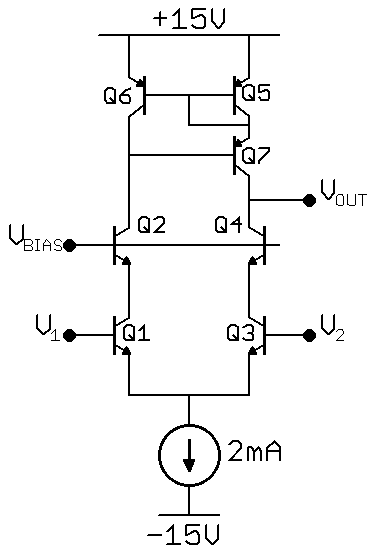
\includegraphics[width=0.4\textwidth]{diff-pair-mirror.png}
\end{center}
	Find $\frac{v_{out}}{v_1-v_2}$ at midband, assuming $\beta_{npn}=200$, 
	$\beta_{pnp}=50$, $V_{A,npn}=100$V, $V_{A,pnp}=50$V, Common-Mode Voltage 
	$V_{CM}=0$, and $V_{BIAS}=4$V.
\clearpage
\subsection*{Problem 2: Op Amp Applications}
	Assume the following circuit is operating at room temperature ($T=300K$)
\begin{center}
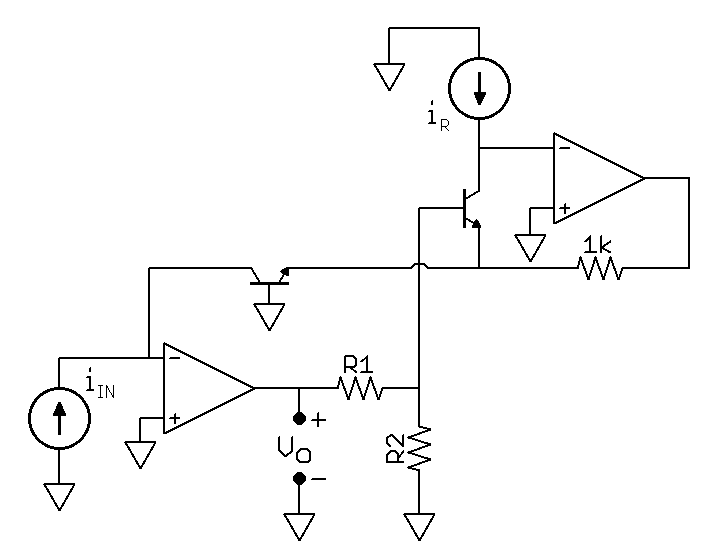
\includegraphics[width=0.7\textwidth]{log-amp.png}
\end{center}
\begin{enumerate}
	\item[(a)] When $R_1=15.7R_2$, $v_o$ is of the form $v_o=A log_{10}(x)$. Find $A$ and $x$.
	\item[(b)] Solve for $R_1$ in terms of $R_2$ such that $v_o=A log_2(x)$ behavior. 
\end{enumerate}

\subsection*{Problem 3: Op Amp Frequency Response}
	The following op amp has a finite gain with frequency response $A(s)=\frac{a_o}{\tau s+1}$ \\
	$a_o=10^6$, $\tau=10^{-6}$, and $f=[1, 0.1, 0.01, 0.001]$.
\begin{center}
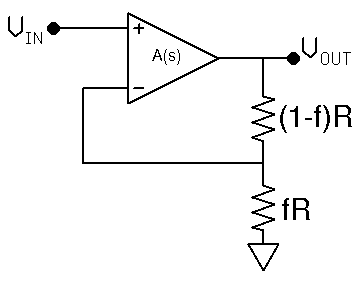
\includegraphics[width=0.35\textwidth]{opamp.png}
\end{center}
\begin{enumerate}
	\item[(a)] Solve for the closed-loop DC gain and upper -3dB frequency for each value of $f$.
	\item[(b)] Sketch the Bode Plot magnitude of $\frac{V_{OUT}}{V_{IN}}(s)$ for each value of $f$ on one plot.
	\item[(c)] What effect does $f$ (gain) have on the step response?
\end{enumerate}

\subsection*{Problem 4: Op Amp Filter}
\begin{center}
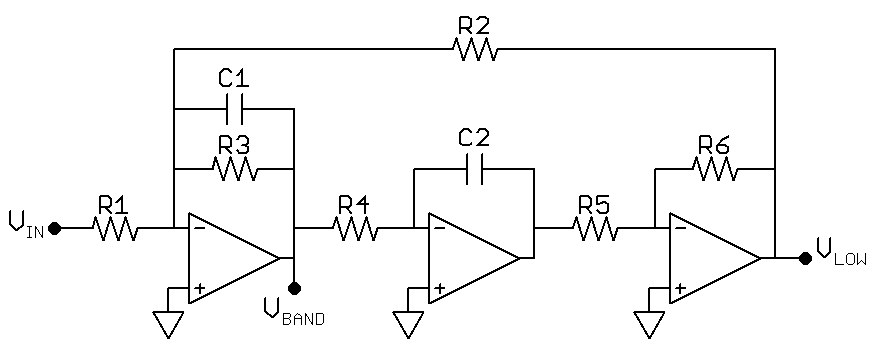
\includegraphics[width=0.7\textwidth]{tow-thomas.png}
\end{center}
Find the transfer functions $\frac{V_{LOW}}{V_{IN}}(s)$ and $\frac{V_{BAND}}{V_{IN}}(s)$ such that the denominator is of the form: 

\begin{equation}
D(s) = s^2+\zeta\omega_os+\omega_o^2
\end{equation}
Find $\zeta$ and $\omega_o$.
\end{document}
